%%%  Chapter 1: Java Program Design and Development
%%%  3rd Edition

%%%REW First draft of chapter 1 - A pdf version sent to Betsy and RAM 12/18/03
%%%RAM Revised draft of chapter 1. Extensive revisions were required in
%%%RAM  reaction to Betsy's edits, were received in early January.
%%%RAM Finished 1/31/03

\setcounter{chapter}{0}
\setcounter{SSTUDYcount}{1}
\chapter{Java Program Design and Development}
\label{ch:intro2}

\CObegin
\secCOBH{Objectives}
\noindent After studying this chapter, you will

\begin{COBL}
\item  Know the basic steps involved in program
       development.
\item  Understand some of the basic elements of the Java language.
\item  Know how to use simple output operations in
       a Java program.
\item  Be able to distinguish between different types of errors in
       a \\program.
\item  Understand how a Java program is translated into
       machine language.
\item  Understand the difference between a Java console application
       and a Java \\Swing application.
\item  Know how to edit, compile, and run Java programs.
\end{COBL}


\secCOLH{Outline}
\begin{COL}
\item Introduction
\item Designing Good Programs
\item Designing a Riddle Program
\item[] {{\color{cyan}Special Topic:} Grace Hopper and the First Computer Bug}
\item Java Language Elements
\item Editing, Compiling, and Running a Java Program
\item From the Java Library: System and PrintStream
\item From the Java Library: {System} and {PrintStream}
\par\small\item[] Chapter Summary
\par\small\item[] Solutions to Self-Study Exercises
\par\small\item[] Exercises
\end{COL}
\COend

\section{Introduction}

\noindent This chapter  introduces some of the basic 
concepts and techniques involved in Java program design and
development.  We begin by identifying the main steps in designing an
object-oriented program. The steps are illustrated by designing a
program that ``asks'' and ``answers'' riddles. As an example of a
riddle, consider the question ``What is black and white and read all
over?''  The answer, of course, is a newspaper.  Following the design
phase, we then focus on the steps involved in coding a Java program,
including the process of editing, compiling, and running a
program. Because Java programs can be text based applications or
window based graphical applications, we describe how the coding process differs for these two
varieties.

Next we begin to familiarize ourselves with Java's extensive class
library by studying its {\tt PrintStream} and {\tt System}
classes.  These classes contain objects and methods that enable us to
print output from a program.  By the end of the chapter you will be
able to design and write a Java application that ``sings'' your
favorite song. 

\section{Designing Good Programs}

\noindent Programming is not simply a question of typing Java code.
Rather, it involves a considerable amount of planning and careful
designing.  Badly designed programs rarely work correctly.  Even
though it is tempting for novice programmers to start entering code
almost immediately, one of the first rules of programming is

\JavaTIP{PROGRAMMING TIP}{}%
{The sooner you begin to type code, the longer the program will take to
finish, because careful design of the program must precede
coding. This is particularly true of object-oriented programs.}

\noindent In other words, the more thought and care you put into
designing a program, the more likely you are to end up with one
that works correctly.  The following subsections provide a brief overview
of the program development process.

\subsection{The Software Engineering Life Cycle}

\noindent Software engineering is the process of designing
and writing software.  The {\it software life cycle} refers to the
different phases involved in the design and development of a computer
program.  Our presentation of examples in the book will focus on four
phases of the overall life cycle. In the {\em specification} phase we
provide a statement of the problem and a detailed description of what
the program will do. In the {\em design} phase we describe the details
of the various classes, methods, and data that will be used in the
program. The {\em implementation} phase refers to the actual coding of
the program into Java.  In the {\em testing} phase we test the
program's performance to make sure it is correct, recoding it or
redesigning it as necessary.

Figure~\ref{fig:progdev} gives a more detailed overview of the program
development process, focusing most of the attention on the design
phase of the software life cycle. It shows that designing an
object-oriented program is a matter of asking the right questions
about the classes, data, and methods that make up the program. 

Overall, the program development process can be viewed as one that
repeatedly applies the divide-and-conquer principle.  That is, most
programming problems can be repeatedly divided until you have a
collection of relatively easy-to-solve subproblems, each of which can
be handled by an object. In this way the program is
\marginnote{Divide and conquer}
divided into a collection of interacting objects. For each object we
design a class. During class design, each object is divided further
into its variables and methods.

\begin{figure}[h]
%\begin{graphic}
%\figa{CHPTR01:1f7.eps}
\figa{chptr01/progdev.eps}%
{An overview of the program development process.}
{fig:progdev}
%\end{graphic}
\end{figure}
%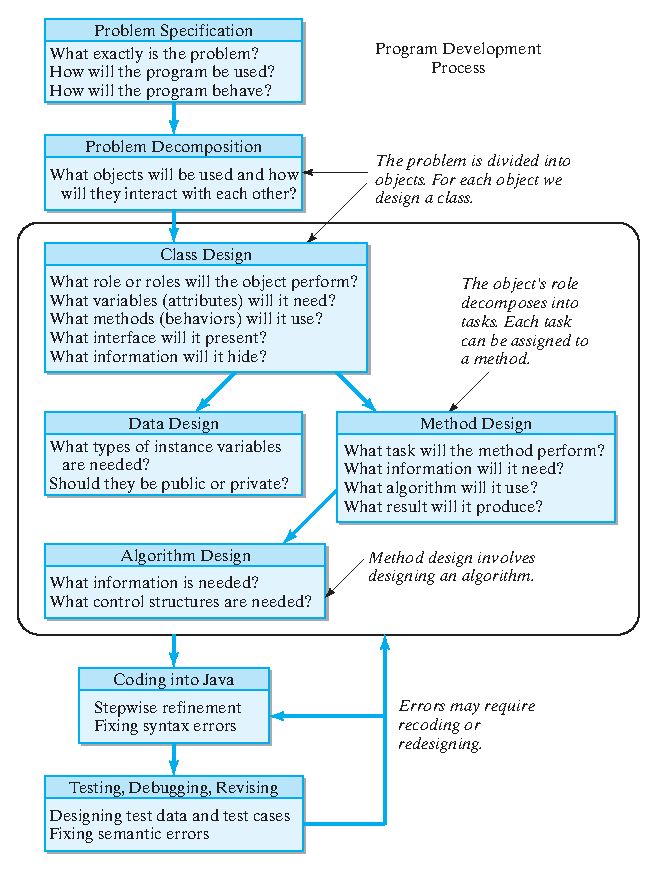
\epsfig{file=ch1-java/figures/progdev.eps}

When should we stop subdividing? How much of a task should be assigned
to a single object or a single method?  The answers to these and
similar questions are not easy.  Good answers require the kind of 
judgment that comes through experience, and frequently there is more
than one good way to design a solution.  Here again, as we learn more
about object-oriented programming, we'll learn more about how to make
these design decisions.

\section{Designing a Riddle Program}

The first step in the program-development process is making sure you
understand the problem (Fig. \ref{fig:progdev}).  Thus, we begin by
developing a detailed specification, which should address three basic
questions:

\begin{BL}
\item  What exactly is the problem to be solved?
\item  How will the program be used?
\item  How should the program behave?
\end{BL}

\noindent In the real world, the problem specification is often
arrived at through an extensive discussion between the customer and
the developer.  In an introductory programming course, the
specification is usually assigned by the instructor.

To help make these ideas a little clearer, let's design an
object-oriented solution to a simple problem.

\BOXDT{{\bf Problem Specification.}
Design a class that will represent a riddle with a given question and
answer.   The definition of this class should make it possible to store
different riddles and to retrieve a riddle's question and answer
independently.
}

\subsection{Problem Decomposition}

\noindent Most problems are too big and too complex to be tackled
all at once. So the next step in the design process is to divide the
\marginnote{Divide and conquer}
problem into parts that make the solution more manageable.  In the
object-oriented approach, a problem is divided into objects, where
each object will handle one specific aspect of the program's overall
job. In effect, each object will become an expert or specialist in
some aspect of the program's overall behavior.

Note that there is some ambiguity here about how far we should go in
decomposing a given program.  This ambiguity is part of the design
process.  How much we should decompose the program before its parts
become ``simple to solve'' depends on the problem we're trying to
solve and on the problem solver.

One useful design guideline for trying to decide what objects
are needed is the following:

\JavaTIP{EFFECTIVE DESIGN}{Looking for Nouns.}{Choosing a program's
objects is often a matter of looking for nouns in the problem
specification.}

\noindent Again, there's some ambiguity involved in this guideline.
For example, the key noun in our current problem is {\it riddle}, so
our solution will involve an object that serves as a model for a
riddle.  The main task of this Java object will be simply to represent
a riddle. Two other nouns in the specification are {\it question} and
{\it answer}. Fortunately, Java has built-in {\tt String} objects that
represent strings of characters such as words or sentences. We can use
two {\tt String} objects for the riddle's question and answer.  Thus,
for this simple problem, we need only design one new type of
object---a riddle---whose primary role will be to represent a riddle's
question and answer.

Don't worry too much if our design decisions seem somewhat mysterious
at this stage. A good understanding of object-oriented design can come
only after much design experience, but this is a good place to start.

\subsection{Object Design}

\noindent Once we have divided a problem into a set of cooperating 
objects, designing a Java program is primarily a matter of designing
and creating the objects themselves. In our example, this means we
must now design the features of our riddle object.  For each object,
we must answer the following basic design questions:

\begin{BL}
\item What role will the object perform in the program?
\vspace{2pt}\item What data or information will it need?
\vspace{2pt}\item What actions will it take?
\vspace{2pt}\item What interface will it present to other objects?
\vspace{2pt}\item What information will it hide from other objects?
\end{BL}

For our riddle object, the answers to these questions are 
shown in Figure~\ref{fig:specs}. Note that although we talk about
``designing an object,'' we are really talking about designing the
object's class. A class defines the collection of objects that belong
to it. The class can be considered the object's {\em type}. This is
the same as for real-world objects. Thus, Seabiscuit is a horse---that
is, Seabiscuit is an object of type horse.  Similarly, an individual
riddle, such as the newspaper riddle, is a riddle.  That is, it is an
object of type Riddle.

The following discussion shows how we arrived at the decisions for the
design specifications for the {\tt Riddle} class, illustrated in
Figure~\ref{fig:specs}.

%%\begin{figure}[tb]
\begin{figure}[h]
\figaproga{100pt}{
\begin{BL}\rm
\item Class Name: Riddle
\item Role: To store and retrieve a question and answer
\item Attributes (Information)
\begin{BSE}
\item question: A variable to store a riddle's question (private)
\item answer: A variable to store a riddle's answer (private)
\end{BSE}
\item Behaviors
\begin{BSE}
\item Riddle(): A method to set a riddle's question and answer
\item getQuestion(): A method to return a riddle's question
\item getAnswer(): A method to return a riddle's answer
\end{BSE}
\end{BL}
}\figaprogb{Design specification for the {\tt Riddle} class.}
%%}\figaprogbleft{Design specification for the {\tt Riddle} class.
{fig:specs}
\end{figure}

The role of the {\tt Riddle} object is to model an ordinary
\marginnote{What is the object's role?}
riddle. Because a riddle is defined in terms of its question and
answer, our {\tt Riddle} object will need some way to store these two
pieces of information. As we learned in Chapter~\ref{chapter-intro}, an instance
variable is a named memory location that belongs to an object. The
fact that the memory location is named, makes it easy to retrieve the
data stored there by invoking the variable's name. For example, to
print a riddle's question we would say something like ``print
question,'' and whatever is stored in {\em question} would be
retrieved and printed.

In general, instance variables are used to store the information that
an object needs to perform its role.
\marginnote{What information will the object need?}
They correspond to what we have been calling the object's
attributes. Deciding on these variables provides the answer to the
question, ``What information does the object need?''  

Next we decide what actions a {\tt Riddle} object will take.
A useful design guideline for actions of objects is the following:

\JavaTIP{EFFECTIVE DESIGN}{Looking for Verbs.}{Choosing the 
behavior of an object is often a matter of looking for verbs in the
problem specification.}

\marginnote{What actions will the object take?}
\noindent For this problem,
the key verbs are {\it set} and {\it retrieve}.  As specified in
Figure~\ref{fig:specs}, each {\tt Riddle} object should provide some
means of setting the values of its question and answer variables and a
means of retrieving each value separately.

Each of the actions we have identified will be encapsulated in a Java
method. As you recall from Chapter~\ref{chapter-intro}, a method is a named section of
code that can be {\em invoked}, or called upon, to perform a
particular action. In the object-oriented approach, calling a method
(method invocation) is the means by which interaction occurs among
objects. Calling a method is like sending a message between
objects. For example, when we want to get a riddle's answer, we
would invoke the {\tt getAnswer()} method.  This is like sending the
message ``Give me your answer.''  One special method, known as a
constructor, is invoked when an object is first created. We will use
the {\tt Riddle()} constructor to give specific values to riddle's
question and answer variables.

In designing an object, we must decide which methods should be made
\marginnote{What interface will it present, and what
information will it hide?}  available to other objects. This
determines what interface the object should present and what
information it should hide from other objects.  In general, those
methods that will be used to communicate with an object are designated
as part of the object's interface. Except for its interface, all other
information maintained by each riddle should be kept ``hidden'' from
other objects. For example, it is not necessary for other objects to
know where a riddle object stores its question and answer. The fact
that they are stored in variables named {\tt question} and {\tt
answer}, rather than variables named {\tt ques} and {\tt ans}, is
irrelevant to other objects.


\JavaTIP{EFFECTIVE DESIGN}{Object Interface.}{An object's interface 
should consist of just those methods needed to communicate with or to
use the object.}

\JavaTIP{EFFECTIVE DESIGN}{Information Hiding.}{An object should 
hide most of the details of its implementation.}


\pagebreak
Taken together, these various design decisions lead to the
\marginfig{chptr01/riddleuml.eps}%
{A UML class diagram representing the  {\tt Riddle} class.}
{fig:ruml}
specification shown in Figure~\ref{fig:ruml}. As our discussion has illustrated,
we arrived at the decisions by asking and answering the right
questions. In most classes the attributes (variables) are
private. This is represented by a minus sign ($-$). In this example,
the operations (methods) are public, which is represented by the plus
sign ($+$). The figure shows that the {\tt Riddle} class has two
hidden (or private) variables for storing data and three visible (or
public) methods that represent the operations that it can perform.

\subsection{Data, Methods, and Algorithms}

\noindent Among the details that must be worked out in
designing a riddle object is deciding what type of data, methods, and
algorithms we need.  There are two basic questions involved:

\begin{BL}
\item  What type of data will be used to represent the information
needed by the riddle?
\item  How will each method carry out its task?
\end{BL}

\noindent Like other programming languages, Java supports a
wide range of different types of data, some simple and some complex.
\marginnote{What type of data will be used?}
Obviously a riddle's question and answer should be represented by
text.  As we noted earlier, Java has a {\tt String} type, which is
designed to store text, which can be considered a string of
characters.

In designing a method, you have to decide what the method will do.  
\marginnote{How will each method carry out its task?}
In order to carry out its task, a method will need certain information,
which it may store in variables.  Plus, it will have to carry out a
sequence of individual actions to perform the task. This is called its
{\bf algorithm}, which is a step-by-step description of the solution
to a problem.  And, finally, you must decide what result the method
will produce.  Thus, as in designing objects, it is important to ask
the right questions:

\begin{BL}
\item  What specific task will the method perform?
\item  What information will it need to perform its task?
\item  What algorithm will the method use?
\item  What result will the method produce?
\end{BL}

\noindent Methods can be thought of as using an algorithm to 
complete a required action.  The algorithm required for the {\tt
Riddle()} constructor is very simple but also typical of constructors
for many classes. It takes two strings and assigns the first to the
{\tt question} instance variable and then assigns the second to the
{\tt answer} instance variable.  The algorithms for the other two
methods for the Riddle class are even simpler.  They are referred to
as {\it get} methods that merely {\it return} or produce the value
that is currently stored in an instance variable.

Not all methods are so simple to design, and not all algorithms are so
\marginnote{Algorithm design}
simple.  Even when programming a simple arithmetic problem, the steps
involved in the algorithm will not always be as obvious as they are
when doing the calculation by hand.  For example, suppose the problem
were to calculate the sum of a list of numbers.  If we were telling our
classmate how to do this problem, we might just say, ``add up all the
numbers and report their total.''  But this description is far too
vague to be used in a program.   By contrast, here's an algorithm that
a program could use:

\begin{NL}
\item  Set the initial value of the sum to 0.
\item  If there are no more numbers to total, go to step 5.
\item  Add the next number to the sum.
\item  Go to step 2.
\item  Report the sum.
\end{NL}

\noindent Note that each step in this algorithm is simple and easy
to follow.   It would be relatively easy to translate it into
Java.  Because English is somewhat imprecise as an algorithmic
language, programmers frequently write algorithms in the programming
\marginnote{Pseudocode}
language itself or in {\bf pseudocode}, a hybrid
language that combines English and programming language structures
without being too fussy about programming language syntax.  For
example, the preceding algorithm might be expressed in pseudocode as
follows:

\begin{jjjlisting}
\begin{lstlisting}
sum = 0
while (more numbers remain)
    add next number to sum
print the sum
\end{lstlisting}
\end{jjjlisting}

Of course, it is unlikely that an experienced programmer would take
the trouble to write out pseudocode for such a simple algorithm.  But
many programming problems are quite complex and require careful design
to minimize the number of errors that the program contains.  In such
situations, pseudocode could be useful.

Another important part of designing an algorithm is to {\it trace}
it---that is, to step through it line by line---on some sample data.
For example, we might test the list-summing algorithm by tracing it on
the list of numbers shown in the margin.
%\begin{table}[h]
%\begin{center}
\marginpar{
\UNTB
\begin{tabular}{rl}
\multicolumn{2}{l}{
\color{cyan}
\rule{8pc}{1pt}}\\[2pt]
%%RAM\UNTBCH{Sum} &\UNTBCH{List of Numbers}
{Sum} & {List of Numbers}
\\[-4pt]\multicolumn{2}{l}{
\color{cyan}
\rule{8pc}{0.5pt}}\\[2pt]
    0        &54 30 20\cr
    54       &30 20\cr
    84       &20\cr
   104       &-
\\[-4pt]\multicolumn{2}{l}{
\color{cyan}
\rule{8pc}{1pt}}
\end{tabular}
\endUNTB
}
%\end{center}
%\end{table}


Initially, the sum starts out at 0 and the
list of numbers contains 54, 30, and 20. On each iteration through the
algorithm, the sum increases by the amount of the next number, and the
list diminishes in size.  The algorithm stops with the correct total
left under the sum column.  While this trace didn't turn up any errors,
it is frequently possible to find flaws in an algorithm by tracing it
in this way.

\subsection{Coding into Java}

\noindent Once a sufficiently detailed design has been developed, it 
is time to start generating Java code.  The wrong way to do this would
be to type the entire program and then compile and run it.  This
generally leads to dozens of errors that can be both demoralizing and
difficult to fix.

The right way to code is to use the principle of {\bf stepwise refinement}. 
\marginnote{Stepwise refinement}
The program is coded in small stages, and after each stage the code is
compiled and tested.  For example, you could write the code for a
single method and test that method before moving on to another part of
the program. In this way, small errors are caught before moving on to
the next stage.

The code for the {\tt Riddle} class is shown in
Figure~\ref{fig:riddleclass}. Even though we have not yet begun
learning the details of the Java language, you can easily pick out the
key parts in this program: the instance variables {\tt question} and
{\tt answer} of type {\tt String}, which are used to store the
riddle's data; the {\tt Riddle()} constructor and the {\tt
getQuestion()} and {\tt getAnswer()} methods make up the interface.
The specific language details needed to understand each of these
elements will be covered in this and the following chapter.

%% proglist ch1/riddle/Riddle.java
\begin{figure}[tb]
\jjjprogstart
\begin{jjjlisting}
\begin{lstlisting}
/*
 * File: Riddle.java
 * Author: Java, Java, Java
 * Description: Defines a simple riddle.
 */
public class Riddle extends Object  // Class header
{                                   // Begin class body
   private String question;       // Instance variables
   private String answer;

   public Riddle(String q, String a) // Constructor method
   {
     question = q;
     answer = a;
   } // Riddle()

   public String getQuestion()   // Instance method
   {
     return question;
   } // getQuestion()

   public String getAnswer()     // Instance method
   {
     return answer;
   } //getAnswer()
} // Riddle class                  // End class body
\end{lstlisting}
\end{jjjlisting}
\jjjprogstop{The {\tt Riddle} class definition.}
{fig:riddleclass}
\end{figure}

\subsection{Syntax and Semantics}
\noindent Writing Java code requires that you know its syntax and 
semantics.  A language's {\bf syntax} is the set of rules
\marginnote{Syntax}
that determines whether a particular statement is correctly
formulated.  As an example of a syntax rule, consider the following
two English statements:


\begin{jjjlisting}
\begin{lstlisting}
The rain in Spain falls mainly on the plain. // Valid
Spain rain the mainly in on the falls plain. // Invalid
\end{lstlisting}
\end{jjjlisting}


\noindent The first sentence follows the rules of English syntax (grammar),
and it means that it rains a lot on the Spanish plain.  The second
sentence does not follow English syntax, and, as a result, it is
rendered meaningless. An example of a Java syntax rule is that a Java
statement must end with a semicolon.

However, unlike in English, where one can still be understood even
when one breaks a syntax rule, in a programming language the syntax
rules are very strict. If you break even the slightest syntax
rule---for example, if you forget just a single semicolon---the
program won't work at all. 


Similarly, the programmer must know the
\marginnote{Semantics}
{\bf semantics} of the language---that is, the meaning of each
statement.  In a programming language, a statement's meaning is
determined by what effect it will have on the program.  For example,
to set the {\tt sum} to 0 in the preceding algorithm, an assignment
statement is used to store the value 0 into the memory location named
{\tt sum}.  Thus, we say that the statement


\begin{jjjlisting}
\begin{lstlisting}
sum = 0;
\end{lstlisting}
\end{jjjlisting}

\noindent assigns 0 to the memory location {\tt sum}, where 
it will be stored until some other part of the program needs it.

Learning Java's syntax and semantics is a major part of learning to
program.  This aspect of learning to program is a lot like learning a
foreign language.  The more quickly you become fluent in the new
language (Java), the better you will be at expressing solutions to
interesting programming problems.  The longer you struggle with Java's
rules and conventions, the more difficult it will be to talk about
problems in a common language.  Also, computers are a lot fussier
about correct language than humans, and even the smallest syntax or
semantic error can cause tremendous frustration.  So, try to be very
precise in learning Java's syntax and semantics.

\subsection{Testing, Debugging, and Revising}

\noindent Coding, testing, and revising a program is an 
repetitive process, one that may require you to repeat the different
program-development stages shown in (Fig.~\ref{fig:progdev}).
According to the stepwise-refinement principle, the process of
developing a program should proceed in small, incremental steps, where
the solution becomes more refined at each step.  However, no matter
how much care you take, things can still go wrong during the coding
process.

A {\it syntax error} is an error that breaks one of Java's syntax
rules. Such errors will be detected by the Java compiler.  Syntax errors 
\marginnote{Syntax errors}
are relatively easy to fix once you understand the error messages
provided by the compiler.  As long as a program contains syntax
errors, the programmer must correct them and recompile the program.
Once all the syntax errors are corrected, the compiler will produce an
executable version of the program, which can then be run.

When a program is run, the computer carries out the steps specified in
the program and produces results.  However, just because a program
runs does not mean that its actions and results are correct.  A
running program can contain {\it semantic errors}, also called 
\marginnote{Semantic errors}
{\it logic errors}.  A semantic error is caused by an error in the
logical design of the program causing it to behave incorrectly,
producing incorrect results.

Unlike syntax errors, semantic errors cannot be detected
automatically.   For example, suppose that a program contains the
following statement for calculating the area of a rectangle:


\begin{jjjlisting}
\begin{lstlisting}
return length + width;
\end{lstlisting}
\end{jjjlisting}

\noindent Because we are adding length and width instead of
multiplying them, the area calculation will be incorrect.  Because
there is nothing syntactically wrong with the expression {\tt length +
width}, the compiler won't detect an error in this statement.  Thus,
the computer will still execute this statement and compute the
incorrect area. 

Semantic errors can only be discovered by testing the program and they
are sometimes very hard to detect. Just because a program appears to
run correctly on one test doesn't guarantee that it contains no
semantic errors. It might just mean that it has not been adequately
tested.

Fixing semantic errors is known as {\it debugging} a program, and when
subtle errors occur it can be the most frustrating part of the whole
program development process.  The various examples presented will
occasionally provide hints and suggestions on how to track down {\it
bugs}, or errors, in your code.  One point to remember when you are
trying to find a very subtle bug is that no matter how convinced you
are that your code is correct and that the bug must be caused by some
kind of error in the computer, the error is almost certainly caused by
your code!

\subsection{Writing Readable Programs}
\noindent Becoming a proficient programmer goes beyond 
simply writing a program that produces correct output.   It also involves 
\marginnote{Programming style}
developing good {\it programming style}, which includes how readable
and understandable your code is.  Our goal is to help you develop a
programming style that satisfies the following principles:

\begin{BL}
\item  {\bf Readability.}
Programs should be easy to read and understand.  Comments should
be used to document and explain the program's code.

\item  {\bf Clarity.}
Programs should employ well-known constructs and standard conventions
and should avoid programming tricks and unnecessarily obscure or
complex code.

\item  {\bf Flexibility.}
Programs should be designed and written so that they are easy to modify.
\end{BL}

\section*{{\color{cyan}Special Topic:} Grace Hopper and \\
\hspace*{20pt}the First Computer Bug}

{\color{cyan}Rear Admiral} Grace Murray Hopper (1906--1992) was a
pioneer computer programmer and one of the original developers of the
COBOL programming language, which stands for {\it CO}mmon {\it
B}usiness-{\it O}riented {\it L}anguage.  Among her many achievements
and distinctions, Admiral Hopper also had a role in coining the term
{\it computer bug}.

In August 1945, she and a group of other programmers were working on
the Mark I, an electro-mechanical computer developed at Harvard that
was one of the ancestors of today's electronic computers.  After
several hours of trying to figure out why the machine was
malfunctioning, someone located and removed a two-inch moth from one
of the computer's circuits.  From then on whenever anything went wrong
with a computer, Admiral Hopper and others would say ``it had bugs in
it.''  The first bug itself is still taped to Admiral Hopper's 1945
log book, which is now in the collection of the Naval Surface Weapons
Center.

In 1991, Admiral Hopper was awarded the National Medal of Technology
by President George Bush.  To commemorate and honor Admiral Hopper's
many contributions, the U.S.~Navy recently named a warship after her.
For more information on Admiral Hopper, see the Web site at

\WWWleft
\begin{jjjlisting}
\begin{lstlisting}[commentstyle=\color{black}\small]
http://www.chips.navy.mil/
\end{lstlisting}
\end{jjjlisting}


\section{Java Language Elements}

\noindent In this section we will introduce some of the key elements 
of the Java language by describing the details of a small program.  We
will look at how a program is organized and what the various parts
do. Our intent is to introduce important language elements, many of
which will be explained in greater detail in later sections.

The program we will study is a Java version of the traditional
HelloWorld program---''traditional'' because practically every
introductory programming text begins with it. When it is run, the
HelloWorld program (Fig.~\ref{fig:helloworld}) just displays the
greeting ``Hello, World!'' on the console.

%% proglist ch1/helloapplication/HelloWorld.java
\begin{figure}[hb]
\jjjprogstart
\begin{jjjlisting}
\begin{lstlisting}[numberstyle=\small,numbers=left]
  /*
   * File: HelloWorld.java
   * Author: Java Java Java
   * Description: Prints Hello, World! greeting.
   */
 public class HelloWorld extends Object // Class header
 {                                   // Start class body
   private String greeting = "Hello, World!";  
   public void greet()               // Method definition
   {                                 // Start method body
       System.out.println(greeting); //  Output statement
   } // greet()                      // End method body
  public static void main(String args[])// Method header
  {                   
    HelloWorld helloworld;         // declare
    helloworld = new HelloWorld(); // create
    helloworld.greet();            // Method call
   }  //  main()
 }  // HelloWorld                  // End class body
\end{lstlisting}
\end{jjjlisting}
\jjjprogstop{The {\tt HelloWorld} application program.}
{fig:helloworld}
\end{figure}


\subsection{Comments}

\noindent The first thing to notice about the {\tt HelloWorld} program 
is the use of comments. A {\bf comment} is a non-executable portion of
a program that is used to document the program. Because comments are
not executable instructions they are just ignored by the compiler.
Their sole purpose is to make the program easier for the programmer to
read and understand.

The {\tt HelloWorld} program contains examples of two types of Java
comments.  Any text contained within /* and */ is considered a
comment.  As you can see in {\tt HelloWorld}, this kind of comment can
extend over several lines and is sometimes called a {\em multiline}
comment.  A second type of comment is any text that follows double
slashes (//) on a line.  This is known as a {\it single-line comment}
because it cannot extend beyond a single line.

When the compiler encounters the beginning marker (/*) of a multiline
comment, it skips over everything until it finds a matching end marker
(*/).  One implication of this is that it is not possible to put one
multiline comment inside of another. That is, one comment cannot be
{\it nested}, or contained, within another comment. The following code
segment illustrates the rules that govern the use of /* and */:


\begin{jjjlisting}
\begin{lstlisting}
/* This first comment begins and ends on the same line. */
/* A second comment starts on this line ...
   and goes on ...
   and this is the last line of the second comment. 
*/ 
/* A third comment starts on this line ...
    /* This is NOT a fourth comment. It is just 
       part of the third comment.
   And this is the last line of the third comment. 
*/
*/  This is an error because it is an unmatched end marker.
\end{lstlisting}
\end{jjjlisting}

\noindent As you can see from this example, it is impossible
to begin a new comment inside an already-started comment because
all text inside the first comment, including /*, is ignored
by the compiler.

\JavaRule{Comments.}{Any text contained within /* and */, which may 
span several lines, is considered a comment and is ignored by the
compiler.  Inserting double slashes (//) into a line turns the rest of
the line into a comment.}

Multiline comments are often used to create a {\em comment block} that
provides useful documentation for the program. In {\tt HelloWorld},
the program begins with a comment block that identifies the name of
file that contains the program and its author and provides a brief
description of what the program does.

For single-line comments, double slashes (//) can be inserted anywhere
\marginnote{Single-line comment}
on a line of code. The result is that the rest of the line is ignored
by the compiler.  We use single-line comments throughout the {\tt
HelloWorld} program to provide a running commentary of its language
elements.

\JavaTIP[false]{PROGRAMMING TIP}{Use of Comments.}%
{A well-written program should begin with a comment block that provides
the name of the program, its author, and a description of what the
program does.}

\subsection{Program Layout}

Another thing to notice about the program is how neatly it is arranged
on the page. This is done deliberately so that the program is easy to
read and understand. In Java, program expressions and statements may
be arranged any way the programmer likes. They may occur one per line,
several per line, or one per several lines.  But the fact that the
rules governing the layout of the program are so lax makes it all the
more important that we adopt a good programming style, one that will
help make programs easy to read.

So look at how things are presented in {\tt HelloWorld}. Notice how
beginning and ending braces, { and }, are aligned, and
note how we use single-line comments to annotate ending braces. Braces
are used to mark the beginning and end of different blocks of code in
a Java program and it can sometimes be difficult to know which
beginning and end braces are matched up. Proper indentation and the
use of single-line comments make it easier to determine how the braces
are matched up.

Similarly, notice how indentation is used to show when one element of
the program is contained within another element. Thus, the elements of
the {\tt HelloWorld} class are indented inside of the braces that mark
the beginning and end of the class. And the statements in the {\tt
main()} method are indented to indicate that they belong to that
method.  Use of indentation in this way, to identify the program's
structure, makes the program easier to read and understand.

\JavaTIP{PROGRAMMING TIP}{Use of Indentation.}
{Indent the code within a block and align the block's opening and closing
braces.  Use a comment to mark the end of a block of code.}

\subsection{Keywords and Identifiers}
\label{subsec:keywords}

\noindent The Java language contains 48 predefined {\it keywords} (Table~\ref{tab:keywords}).
These are words that have special meaning in the language and whose
use is reserved for special purposes. For example, the keywords used
in the HelloWorld program (Fig.~\ref{fig:helloworld}) are: {\tt
class}, {\tt extends}, {\tt private}, {\tt public}, {\tt static}, and
{\tt void}. 

\begin{table}[htb]
%\hphantom{\caption{Java keywords}}
{\caption{Java keywords.\label{tab:keywords}}}
%\begin{tabular}{l}
{\color{cyan}\rule{27pc}{1pt}}\par\vspace{-10pt}
\begin{verbatim}
abstract   default   goto             package       this
boolean    do        if               private       throw
break      double    implements       protected     throws
byte       enum      import           public        transient
case       elses     instanceof       return        try
catch      extend    int              short         void
char       final     interface        static        volatile
class      finally   long             super         while
const      float     native           switch
continue   for       new              synchronized
\end{verbatim}
\par\vspace{-14pt}{\color{cyan}\rule{27pc}{1pt}}
%\end{tabular}
\endTB
\end{table}

Because their use is restricted, keywords cannot be used as the names
of methods, variables, or classes.  However, the programmer can make
up his or her own names for the classes, methods, and variables that
occur in the program, provided that certain rules and conventions are
followed.

The names for classes, methods, and variables are called identifiers,
\marginnote{Identifier syntax}
which follow certain syntax rules:

\JavaRule[false]{Identifier.}{ An {\bf identifier} must begin
with a capital or lowercase letter and may be followed by any number
of letters, digits, underscores (\_), or dollar signs (\$). An
identifier may not be identical to a Java keyword.}

\noindent Names in Java are {\it case sensitive}, which means that
two different identifiers may contain the same letters in the same
order. For example, {\tt thisVar} and {\tt ThisVar} are two different
identifiers.

In addition to the syntax rule that governs identifiers, Java
\marginnote{Identifier style}
programmers follow certain style conventions in making up names for
classes, variables, and methods. By convention, class names in Java
begin with a capital letter and use capital letters to distinguish the
individual words in the name---for example, {\tt HelloWorld} and {\tt
\marginnote{Java naming conventions}
TextField}.  Variable and method names begin with a lowercase letter
but also use capital letters to distinguish the words in the
name---for example, {\tt main()}, {\tt greeting}, {\tt greet()}, {\tt
getQuestion()}, and {\tt getAnswer()}.  The advantage of this convention
is that it is easy to distinguish the different elements in a
program---classes, methods, variables---just by how they are
written. (For more on Java style conventions, see
Appendix A.).

Another important style convention followed by Java programmers
is to choose descriptive identifiers when naming classes,
variables, and methods. This helps to make the program more
readable.

\JavaTIP{PROGRAMMING TIP}{Choice of Identifiers.}%
{To make your program more readable, choose names that describe the
purpose of the class, variable, or method.}

\subsection{Data Types and Variables}
\label{subsec:primitives}


\noindent A computer program wouldn't be very useful if it couldn't
manipulate different kinds of data, such as numbers and strings.  The
operations that one can do on a piece of data depend on the data's
type. For example, you can divide and multiply numbers, but you cannot
do this with strings.  Thus, every piece of data in a Java program is
classified according to its {\bf data type}.

Broadly speaking, there are two categories of data in Java: various
types of objects and eight different types of built-in {\bf primitive
data types}.  In addition to new types of objects that are created by
programmers, Java has many different types of built-in objects. Two
types that we will encounter in this chapter are the {\tt String} and
{\tt PrintStream} objects. Java's primitive types include three
\marginnote{Primitive types}
integer types, three real number types, a character type, and a
boolean type with values true and false.  The names of the primitive
types are keywords like {\tt int} for one integer type, {\tt double}
for one real number type, and {\tt boolean}.

As we noted in Chapter~\ref{chapter-intro}, a variable is a named storage location that
can store a value of a particular type. Practically speaking, you can
think of a variable as a special container into which you can place
values, but only values of a certain type (Fig.~\ref{fig:vars}). For
example, an {\tt int} variable can store values like 5 or -100. A {\tt
String} variable can store values like ``Hello''.  (Actually, this is
not the full story, which is a little more complicated, but we will
get to that in Chapter~\ref{chapter-objects}.)

In the {\tt HelloWorld} class, the instance variable {\tt greeting}
\marginfig{chptr01/vars.eps}{Variables are like {\it typed} containers.}
{fig:vars}
(line 8) stores a value of type {\tt String}. In the {\tt main()}
method, the variable {\tt helloworld} is assigned 
a {\tt HelloWorld} object (line 16).

A {\bf literal value} is an actual value of some type that occurs in a
program. For example, a string enclosed in double quotes, such as
"Hello, World!", is known as a {\tt String} literal. A number such as
45.2 would be an example of a literal of type {\tt double}, and -72
would be an example of a literal of type {\tt int}.  Our HelloWorld
program contains just a single literal value, the "HelloWorld!" {\tt
String}.

\subsection{Statements}
\label{subsec:statements}

A Java program is a collection of statements. A {\bf statement} is a
\marginnote{Executing a program}
segment of code that takes some action in the program. As a program runs,
we say it {\em executes} statements, meaning it carries out the actions
specified by those statements.  In our {\tt HelloWorld} program, statements
of various types occur on lines 8, 11, 15, 16, and 17. Notice that all
of these lines end with a semicolon. The rule in Java is that statements
must end with a semicolon. Forgetting to do so would cause a syntax error.

A {\bf declaration statement} is a statement that declares a variable
of a particular type. In Java, a variable must be declared before it
can be used in a program. Failure to do so would cause a syntax error.
In its simplest form, a declaration statement begins with the
\marginnote{Declaration statement}
variable's type, which is followed by the variable's name, and ends
with a semicolon:

\begin{extract}
{\it Type VariableName} ;
\end{extract}

\noindent A variable's type is either one of the primitive types
we mentioned, such as {\tt int}, {\tt double}, or {\tt boolean}, or
for objects, it is the name of the object's class, such as {\tt
String} or {\tt HelloWorld}. A variable's name may be any legal
identifier, as defined earlier, although the convention in Java is to
begin variable names with a lowercase letter.  In our {\tt HelloWorld}
program, an example a simple declaration statement occurs on line 15:

\begin{jjjlisting}
\begin{lstlisting}
HelloWorld helloworld;                    
\end{lstlisting}
\end{jjjlisting}

\noindent This example declares a variable for an
object.  The variable's name is {\tt helloworld} and its type is {\tt
HelloWorld}, the name of the class that is being defined in our
example.  To take another example the following statements declare two
{\tt int} variables, named {\tt int1} and {\tt int2}:

\begin{jjjlisting}
\begin{lstlisting}
int int1; 
int int2;
\end{lstlisting}
\end{jjjlisting}

\noindent As we noted, an {\tt int} is one of Java's primitive types
and the word {\it int} is a Java keyword. 

Without going into too much detail at this point, declaring a
variable causes the program to set aside enough memory for the type of
data that will be stored in that variable. So in this example, Java
would reserve enough space to store an {\tt int}.

An {\bf assignment statement} is a statement that stores (assigns) a
value in a variable.  An assignment statement uses the equal sign ($=$)
as an assignment operator. In its simplest form, an assignment
statement has a variable on the left hand side of the equals sign and
some type of value on the right hand side. Like other statements, an
assignment statement ends with a semicolon:

\begin{extract}
{\it VariableName} = {\it Value} ;
\end{extract}

\noindent When it executes an assignment statement, Java will first
determine what value is given on the right hand side and then
assign (store) that value to (in) the variable on the left hand
side. Here are some simple examples:
\marginfig{chptr01/assign.eps}{This illustrates how the state of the 
variables {\tt num1} and {\tt num2} changes over the course of
the three assignments, (a), (b), (c), given in the text.}
{fig:assign}

\begin{jjjlisting}
\begin{lstlisting}
greeting = "Hello, World";
num1 = 50;        // (a) Assign 50 to num1
num2 = 10 + 15;   // (b) Assign 25 to num2
num1 = num2;      // (c) Copy num2's value (25) into num1
\end{lstlisting}
\end{jjjlisting}

\noindent In the first case, the value on the right hand 
side is the string literal "Hello, World!", which gets stored in {\tt
greeting}. Of course, {\tt greeting} has to be the right type of
container--in this case, a {\tt String} variable.  In the next case,
the value on the right hand side is 50. So that is the value that gets
stored in {\tt num1}, assuming that {\tt num1} is an {\tt int}
variable. The situation after this assignment is shown in the top
drawing in Figure~\ref{fig:assign}.  In the third case, the value on
the right hand side is 25, which is determined by adding 10 and 15. So
the value that gets assigned to {\tt num2} is 25. After this
assignment we have the situation shown in the middle drawing in the
figure. Of course, this assumes that {\tt num2} is an {\tt int}
variable.  In the last case, the value on the right hand side is 25,
the value that we just stored in the variable {\tt num2}. So, 25 gets
stored in {\tt num1}. This is the bottom drawing in the accompanying
figure.

The last of these examples 

\begin{jjjlisting}
\begin{lstlisting}
num1 = num2;   // Copy num2's value into num1
\end{lstlisting}
\end{jjjlisting}

\noindent can be confusing to beginning programmers, so it is worth
some additional comment. In this case, there are variables on both the
left and right of the assignment operator. But they have very
different meaning. The variable on the right is treated as a value. If
that variable is storing 25, then that is its value. In fact, whatever
occurs on the right hand side of an assignment operator is treated as
a value. The variable on the left hand side is treated as a memory
location. It is where the value 25 will be stored as a result of
executing this statement. The effect of this statement is to copy
the value stored in {\it num2} into {\it num1}, as illustrated
\marginfig{chptr01/assign2.eps}{In the 
assignment {\it num1 = num2;},  {\it num2}'s
value is copied into {\it num1}.}
{fig:assign2}
in Figure~\ref{fig:assign2}.

Java has many other kinds of statements and we will be learning about
these in subsequent examples. The following examples from the {\tt
HelloWorld} program are examples of statements in which a method
is called:

\begin{jjjlisting}
\begin{lstlisting}
System.out.println(greeting);// Call println() method
helloworld.greet();          // Call greet() method
\end{lstlisting}
\end{jjjlisting}

\noindent We will discuss these kinds of statements in greater 
detail as we go along. One final type of statement that should be
mentioned at this point is the {\bf compound statement} (or {\bf
block}), which is a sequence of statements contained within braces
({}).  We see three examples of this in the {\tt
HelloWorld} program. The body of a class definition extends from lines
7 through 19. The body of the {\tt greet()} method is a block that
extends from lines 10 through 12. The body of the {\tt main()} method
is a block that extends from lines 14 to 19.

\subsection{Expressions and Operators}
\label{subsec:expressions}

\noindent The manipulation of data in a program is done by using some
kind of {\em expression} that specifies the action.  An {\bf
expression} is Java code that specifies or produces a value in the
program.  For example, if you want to add two numbers, you would use
an arithmetic expression, such as $num1 + num2$. If you want to
compare two numbers, you would use a relation expression such as $num1
< num2$. As you can see, these and many other expressions in Java
involve the use of special symbols called {\bf operators}. Here we see
the addition operator ($+$) and the less-than operator ($<$). We have
already talked about the assignment operator ($=$).

Java expressions and operators have a type that depends on the type of
data that is being manipulated. For example, when adding two {\tt int}
values, such as $5 + 10$, the expression itself produces an {\tt int}
result.  When comparing two numbers with the less than operator, $num1
< num2$, the expression itself produces a {\tt boolean} type, either
true or false. 

It is important to note that expressions cannot occur on their own.
Rather they occur as part of the program's statements.  Here are some
additional examples of expressions:

\begin{jjjlisting}
\begin{lstlisting}
num = 7      // An assignment expression of type int
num = square(7) // An method call expression of type int
num == 7     // An equality expression of type boolean
\end{lstlisting}
\end{jjjlisting}

\noindent  The first of these is an assignment expression. It has a value 
of {\tt 7}, because it is assigning {\tt 7} to {\tt num}. The second
example is also an assignment expression, but this one has a method
call, {\tt square(7)}, on its right hand side. (We can assume that a
method named {\tt square()} has been appropriately defined in the
program.)  A method call is just another kind of expression. In this
case, it has the value 49.  Note that an assignment expression can be
turned into a stand-alone assignment statement by placing a semicolon
after it.

The third expression is an equality expression, which has the value
{\tt true}, assuming that the variable on its left is storing the
value 7. It is important to note the difference between the assignment
operator ($=$) and the equality operator ($==$).

\JavaRule{Equality and Assignment.} {Be careful not to
confuse {\tt =} and {\tt ==}. The symbol {\tt =} is the assignment
operator. It assigns the value on its right-hand side to the variable
on its left-hand side. The symbol {\tt ==} is the equality
operator. It evaluates whether the expressions on its left- and
right-hand sides have the same value and returns either {\tt true} or
{\tt false}.}

\secEXRHone{Self-Study Exercises}
\begin{SSTUDY}

\item What is stored in the variable {\tt num} after the following
two statements are executed?
\small
\begin{verbatim}
  int num = 11;
  num = 23 - num;
\end{verbatim}
\normalsize

\item Write a statement that will declare a variable of type {\tt int}
called {\tt num2}, and store in it the sum of 711 and 712. 

\end{SSTUDY}


\subsection{Class Definition}

\noindent A Java program consists of one or more class definitions. 
In the {\tt HelloWorld} example, we are defining the {\tt HelloWorld}
class, but there are also three predefined classes involved in the
program. These are the {\tt Object}, {\tt String}, and {\tt System}
classes all of which are defined in the Java class library. Predefined
classes, such as these, can be used in any program.

As the {\tt HelloWorld} program's comments indicate, a class definition
\marginnote{Class header}
has two parts: a {\it class header} and a {\it class body}.  In
general, a class header takes the following form, some parts of which
are optional ({\em opt}):
$$
\hbox{\it ClassModifiers}_{\hbox{\scriptsize\it opt}}\quad
\hbox{\tt class}\quad
\hbox{\it ClassName}\quad
\hbox{\it Pedigree}_{\hbox{\scriptsize\it opt}}
$$

\noindent The class header for the {\tt HelloWorld} class is:

\begin{jjjlisting}
\begin{lstlisting}
public class HelloWorld extends Object
\end{lstlisting}
\end{jjjlisting}

\noindent The purpose of the header is to give the class its name 
({\tt HelloWorld}), identify its accessibility ({\tt public} as
opposed to {\tt private}), and describe where it fits into the Java class
hierarchy (as an extension of the {\tt Object} class). In this case,
the header begins with the optional access modifier, {\tt public},
which declares that this class can be accessed by any other
classes. The next part of the declaration identifies the name of the
class, {\tt HelloWorld}. And the last part declares that {\tt
HelloWorld} is a subclass of the {\tt Object} class. We call this
part of the definition the class's pedigree.

As you recall from Chapter~\ref{chapter-intro}, the {\tt Object} class is the top class
of the entire Java hierarchy. By declaring that {\tt HelloWorld
extends Object}, we are saying that {\tt HelloWorld} is a direct {\em
subclass} of {\tt Object}.  In fact, it is not necessary to declare
explicitly that {\tt HelloWorld} extends {\tt Object} because that is
Java's default assumption. That is, if you omit the extends clause in
the class header, Java will automatically assume that the class is a
subclass of {\tt Object}.

The class's body, which is enclosed within curly brackets ({}),
\marginnote{Class body}
contains the declaration and definition of the elements that make up
the objects of the class.  This is where the object's attributes and
actions are defined. 

\subsection{Declaring an Instance Variable}
\label{subsec:vardecl}

There are generally two kinds of elements declared and defined in the
class body: variables and methods. As we described in Chapter~\ref{chapter-intro}, an
instance variable is a variable that belongs to each object, or
instance, of the class. That is, each instance of a class has its own
copies of the class's instance variables.  The {\tt HelloWorld} class
has a single instance variable, ({\tt greeting}), which is declared as
follows:

\begin{jjjlisting}
\begin{lstlisting}
private String greeting = "Hello, World!"; 
\end{lstlisting}
\end{jjjlisting}

\noindent In general, an instance variable declaration has the following
syntax, some parts of which are optional:

$$
\hbox{\it Modifiers}_{\hbox{\scriptsize\it opt}}\quad
\hbox{\it Type}\quad
\hbox{\it VariableName}\quad
\hbox{\it InitializerExpression}_{\hbox{\scriptsize\it opt}}
$$

\noindent Thus, a variable declaration begins with optional modifiers. 
In declaring the {\tt greeting} variable, we use the access modifier,
{\tt private}, to declare that {\tt greeting}, which belongs to the
{\tt HelloWorld} class, cannot be directly accessed by other
objects. The next part of the declaration is the variable's type. In
\marginnote{Information hiding}
this case, the {\tt greeting} variable is a {\tt String}, which means
that it can store a string object.  The type is followed by the name
of the variable, in this case ({\tt greeting}). This is the name that
is used to refer to this memory location throughout the class. For
example, notice that the variable is referred to on line 11 where it
is used in a {\tt println()} statement.

The last part of the declaration is an optional initializer
expression. In this example, we use it to assign an initial value,
``Hello, World!,'' to the {\tt greeting} variable.  

\subsection{Defining an Instance Method}

Recall that a method is a named section of code that can be called or
invoked to carry out an action or operation.  In a Java class, the
methods correspond to the object's behaviors or actions. The {\tt
HelloWorld} program has two method definitions: the {\tt greet()}
method and the {\tt main()} method.

A method definition consists of two parts: the method header and the
method body. In general, a method header takes the following
form, including some parts which are optional:

$$
\hbox{\it Modifiers}_{\hbox{\scriptsize\it opt}}\quad
\hbox{\it ReturnType}\quad
\hbox{\it MethodName}\quad
\hbox{\tt (}\quad
\hbox{\it ParameterList}_{\hbox{\scriptsize\it opt}}
\hbox{\tt )}\quad
$$

\noindent As with a variable declaration, a method definition
begins with optional modifiers. For example, the definition of the
{\tt greet()} method on line 9 uses the access modifier, {\tt public},
to declare that this method can be accessed or referred to by other
classes.  The {\tt main()} method, whose definition begins on line 13,
is a special method, and is explained in the next section.

The next part of the method header is the method's return type. This
is the type of value, if any, that the method returns.  Both of the
methods in {\tt HelloWorld} have a return type of {\tt void}. This
means that they don't return any kind of value. Void methods just
execute the sequence of statements given in their bodies.  For an
example of a method that does return a value, take a look again at the
declaration of the {\tt getQuestion()} method in the {\tt Riddle}
class, which returns a {\tt String} (Fig.~\ref{fig:riddleclass}).

The method's name follows the method's return type. This is the name
that is used when the method is called. For example, the {\tt greet()}
method is called on line 17.

Following the method's name is the method's parameter list. A {\bf
parameter} is a variable that temporarily stores data values that are
being passed to the method when the method is called. Some methods,
such as the {\tt greet()} method, do not have parameters, because they
are not passed any information. For an example of a method that does
have parameters, see the {\tt Riddle()} constructor, which contains
parameters for the riddle's question and answer
(Fig.~\ref{fig:riddleclass}).  

The last part of method definition is its body, which contains a
sequence of executable statements. An {\bf executable statement} is a
Java statement that takes some kind of action when the program is run.
For example, the statement in the {\tt greet()} method,

\begin{jjjlisting}
\begin{lstlisting}
System.out.println(greeting);   //  Output statement
\end{lstlisting}
\end{jjjlisting}

\noindent prints a greeting on the console. 

\subsection{Java Application Programs}

The HelloWorld program is an example of a Java {\bf application
program}, or a Java application, for short.  An application program is
a stand-alone program, ``stand-alone'' in the sense that it does not
depend on any other program, like a Web browser, for its execution.
Every Java application program must contain a {\tt main()} method,
which is where the program begins execution when it is run. For a
program that contains several classes, it is up to the programmer to
decide which class should contain the {\tt main()} method. We don't
have to worry about that decision for the HelloWorld, because it
contains just a single class.

Because of its unique role as the starting point for every
Java application program,  it is very important that the header for
the main method be declared exactly as shown in the {\tt HelloWorld}
class:

\begin{jjjlisting}
\begin{lstlisting}
public static void main(String args[])   
\end{lstlisting}
\end{jjjlisting}

\noindent It must be declared {\tt public} so it can be accessed
from outside the class that contains it.  The {\tt static} modifier
\marginnote{Class method}
is used to designate {\tt main()} as a class method. As you might
recall from Chapter 0, a class method is a method that is associated
directly with the class that contains it rather than with the objects
of the class. A class method is not part of the class's
objects. Unlike instance methods, which are invoked through a class's
objects, a class method is called through the class itself. Thus, a
class method can be called even before the program has created objects
of that class. Because of {\tt main()}'s special role as the program's
starting point, it is necessary for {\tt main()} to be a class method
because it is called, by the Java runtime system, before the program
has created any objects.

The {\tt main()} method has a {\tt void} return type, which means it
does not return any kind of value. Finally, notice that {\tt main()}'s
parameter list contains a declaration of some kind of {\tt String}
parameter named {\it args}. This is actually an array that can be used
to pass string arguments to the program when it is started up. We
won't worry about this feature until our chapter on arrays.

\subsection{Creating and Using Objects}

\noindent The body of the {\tt main()} method is where the 
{\tt HelloWorld} program creates its one and only object.  Recall that
when it is run the {\tt HelloWorld} program just prints the ``Hello
World!'' greeting. As we noted earlier, this action happens in the
{\tt greet()} method. So in order to make this action happen, we need
to call the {\tt greet()} method. However, because the {\tt greet()}
method is an instance method that belongs to a {\tt HelloWorld}
object, we first need to create a {\tt HelloWorld} instance. This is
what happens in the body of the {\tt main()} method
(Fig.~\ref{fig:helloworld}).

The {\tt main()} method contains three statements:

\begin{jjjlisting}
\begin{lstlisting}
HelloWorld helloworld;          // Variable declaration
helloworld = new HelloWorld();  // Object instantiation
helloworld.greet();             // Method invocation
\end{lstlisting}
\end{jjjlisting}

\noindent The first statement declares a variable of type 
{\tt HelloWorld}, which is then assigned a {\tt HelloWorld} object. 
The second statement creates a {\tt HelloWorld}
object. This is done by invoking the {\tt HelloWorld()} constructor
method. Creating an object is called {\bf object instantiation}
because you are creating an instance of the object.  Once a {\tt
HelloWorld} instance is created, we can use one of its instance
methods to perform some task or operation. Thus, in the third
statement, we call the {\tt greet()} method, which will print ``Hello
World!'' on the console.

If you look back at the {\tt HelloWorld} program in
Figure~\ref{fig:helloworld} you won't find a definition of a
\marginnote{Default constructor}
constructor method.  This is not an error because Java will provide a
default constructor if a class does not contain a constructor
definition. The {\bf default constructor} is a trivial constructor
method, ``trivial'' because its body contains no statements. Here
is what the default {\tt HelloWorld()} constructor would look like:

\begin{jjjlisting}
\begin{lstlisting}
public HelloWorld() {  }  // Default constructor
\end{lstlisting}
\end{jjjlisting}

\noindent For most of the classes we design, we will design our
own constructors, just as we did in the {\tt Riddle} class
(Fig.~\ref{fig:riddleclass}).  We will use constructors to assign
initial values to an object's instance variables or to perform other
kinds of tasks that are needed when an object is created. Because the
{\tt HelloWorld} object doesn't require any startup tasks, we can make
do with the default constructor.

The {\tt HelloWorld} program illustrates the idea that an
\marginnote{Interacting objects}
object-oriented program is a collection of interacting objects.
Although we create just a single {\tt HelloWorld} object in the {\tt
main()} method, there are two other objects used in the program. One
is the {\tt greeting}, which is a {\tt String} object consisting of
the string ``Hello, World!''.  The other is the {\tt System.out}
object, which is a special Java system object used for printing.
	
\subsection{Java JFrames}

Java cann run a program in a {\bf JFrame} so that the output 
and interaction occurs in a Window (or Frame). Figure~\ref{fig:hellojframe} shows a Java program named {\tt
HelloWorldSwing}. This program does more or less the same thing as
%% proglist ch1/hellojframe/HelloWorldSwing.java
\begin{figure}[h!]
\jjjprogstart
\begin{jjjlisting}
\begin{lstlisting}
 /** File: HelloWorldSwing program */

import javax.swing.JFrame; // Import class names
import java.awt.Graphics;
import java.awt.Canvas;

public class HelloWorldCanvas extends Canvas // Class header
{                                            
    // Start of body
    public void paint(Graphics g)           
        // The paint method
    {
        g.drawString("Hello, World!", 10, 10);
    }  // End of paint

    public static void main(String[] args){
        HelloWorldCanvas c = new HelloWorldCanvas();
        JFrame f = new JFrame();
        f.add(c);
        f.setSize(150,50);
        f.setVisible(true);
    }
}  // End of HelloWorldCanvas

\end{lstlisting}
\end{jjjlisting}
\jjjprogstop{{\tt Hello\-World\-Canvas} program.}
{fig:hellojframe}
\end{figure}
the {\tt HelloWorld} application---it displays the ``Hello, World!'' 
greeting. The difference is that it displays the greeting within
a Window rather than directly on the console. 

As in the case of the {\tt HelloWorld} console application program, {\tt
Hello\-World\-Canvas} consists of a class definition.  It contains a
single method definition, the {\tt paint()} method, which
contains a single executable statement:

\begin{jjjlisting}
\begin{lstlisting}
g.drawString("Hello, World!",10,10);
\end{lstlisting}
\end{jjjlisting}

\noindent This statement displays the ``Hello, World!'' message
directly in a Window. 
The {\tt drawString()} method is one of the many
drawing and painting methods defined in the {\tt Graphics} class.
Every Java Canvas comes with its own {\tt Graphics} object, which is
referred to here simply as {\tt g}. Thus, we are using that object's
{\tt drawString()} method to draw on the window. Don't worry
if this seems a bit mysterious now. We'll explain it more fully when
we take up graphics examples again.


The {\tt HelloWorldSwing} also contains some elements, such as the
{\tt import} statements, that we did not find in the {\tt HelloWorld}
application. We will now discuss those features.


\subsection{Java Library Packages} 

Recall that the {\tt HelloWorld} application program used two
pre-defined classes, the {\tt String} and the {\tt System}
classes. Both of these classes are basic language classes in Java.
The {\tt HelloWorldSwing} program also uses pre-defined classes, such
as {\tt JFrame} and {\tt Graphics}. However, these two classes are not
part of Java's basic language classes.  To understand the difference
between these classes, it will be necessary to talk briefly about
how the Java class library is organized.

A {\bf package} is a collection a inter-related classes in the Java
class library. For example, the {\tt java.lang} package contains
classes, such as {\tt Object}, {\tt String}, and {\tt System}, that
are central to the Java language. Just about all Java programs use
classes in this package. The {\tt java.awt} package provides classes,
such as {\tt Button}, {\tt TextField}, and {\tt Graphics}, that are
used in graphical user interfaces (GUIs).  The {\tt java.net} package
provides classes used for networking tasks, and the {\tt java.io}
package provides classes used for input and output operations.

All Java classes belong to some package, including those that are
programmer defined. To assign a class to a package, you would provide
a {\tt package} statement as the first statement in the file that
contains the class definition. For example, the files containing the
definitions of the classes in the {\tt java.lang} package all begin
with the following statement.

\begin{jjjlisting}
\begin{lstlisting}
package java.lang;
\end{lstlisting}
\end{jjjlisting}

\noindent If you omit {\tt package} statement, as we do for the
programs in this book, Java places such classes into an unnamed
default package. 

Thus, for any Java class, its full name includes the name of the
package that contains it. For example, the full name for the {\tt
System} class is {\tt java.lang.System} and the full name for the {\tt
String} class is {\tt java.lang.String}.  Similarly, the full name for
the {\tt Graphics} class is {\tt java.awt.Graphics}.  In short, the
full name for a Java class takes the following form:

$$
\hbox{\it package.class}\quad
$$

\noindent In other words, the full name of any class provides
its package name as a prefix.

Of all the packages in the Java library, the {\tt java.lang} package
is the only one whose classes are available by their shorthand names
to all Java programs. This means that when a program uses a class from
the {\tt java.lang} package, it can refer to it simply by its class
name. For example, in the {\tt HelloWorld} program we referred
directly to the {\tt String} class rather than to {\tt
java.lang.String}.

\subsection{The {\tt import} Statement}

The {\tt import} statement makes Java classes available to programs
under their abbreviated names. Any public class in the Java class
library is available to a program by its fully qualified name.  Thus,
if a program was using the {\tt Graphics} class, it could always refer
to it as {\tt java.awt.Graphics}.  However, being able to refer to
{\tt Graphics} by its shorthand name, makes the program a bit
shorter and more readable.

The {\tt import} statement doesn't actually load classes into the
program. It just makes their abbreviated names available.  For
example, the import statements in {\tt HelloWorldSwing} allow us to
refer to the {\tt JFrame}, {\tt Canvas}, and {\tt Graphics} classes by their
abbreviated names (Fig.~\ref{fig:hellojframe}).

The {\tt import} statement takes two possible forms:
$$
\hbox{\tt import }\quad
\hbox{\it package.class}\quad
$$
$$
\hbox{\tt import }\quad
\hbox{\it package.*}\quad\\
$$

\noindent The first form allows a specific class to be known
by its abbreviated name. The second form, which uses the asterisk as a
wildcard characters ('*'), allows all the classes in the specified
package to be known by their short names. The {\tt import} statements
in {\tt HelloWorldSwing} are examples of the first form. The
following example,

\begin{jjjlisting}
\begin{lstlisting}
import java.lang.*;
\end{lstlisting}
\end{jjjlisting}

\noindent allows all classes in the {\tt java.lang} package to
be referred to by their class names alone. In fact, this particular
{\tt import} statement is implicit in every Java program.

\subsection{Qualified Names in Java}
\label{subsec:qualifiednames}

\noindent In the previous subsections we have seen several
examples of names in Java programs that used {\it dot notation}.  A
{\bf qualified name} is a name that is separated into parts using
Java's dot notation. Examples include package names, such as {\tt
java.awt}, class names, such as {\tt javax.swing.JFrame}, and
even method names, such as {\tt helloworld.greet()}.

Just as in our natural language, the meaning of a name within a Java
program depends on the context.  For example, the expression {\tt
helloworld.greet()} refers to the {\tt greet()} method, which
belongs to the {\tt HelloWorld} class.  If we were using this
expression from within that class, you wouldn't need to qualify
the name in this way.  You could just refer to {\tt greet()} and it
would be clear from the context which method you meant.

This is no different than using someone's first name (``Kim'') when
there's only one Kim around, but using a full name (``Kim Smith'')
when the first name alone would be too vague or ambiguous.

One thing that complicates the use of qualified names is that they are
used to refer to different kinds of things within a Java program.  But
this is no different, really, than in our natural language, where
names (``George Washington'') can refer to people, bridges,
universities, and so on. Here again, just as in our natural language,
Java uses the context to understand the meaning of the name.  For
example, the expression {\tt java.lang.System} refers to the {\tt
System} class in the {\tt java.lang} package, whereas the expression
{\tt System.out.print()} refers to a method in the {\tt System.out}
object.

How can you tell these apart?  Java can tell them apart because the
first one occurs as part of an {\tt import} statement, so it must be
referring to something that belongs to a package.  The second expression
would only be valid in a context where a method invocation is allowed.
You will have to learn a bit more about the Java language before
you'll be able to completely understand these names, but the following
provide some naming rules to get you started.

\JavaRule{Library Class Names.}{By convention, class
names in Java begin with an uppercase letter.  When referenced as part
of a package, the class name is the last part of the name.  For
example, {\tt java.lang.System} refers to the {\tt System} class in
the {\tt java.lang} package.}

\JavaRule{Dot Notation.}{Names expressed in Java's
{\it dot notation} depend for their meaning on the context in which
they are used.  In qualified names---that is, names of the form
X.Y.Z---the last item in the name (Z) is the {\it referent}---that is,
the element being referred to.  The items that precede it (X.Y.) are
used to qualify or clarify the referent.}

\noindent The fact that names are context dependent in this way certainly
complicates the task of learning what's what in a Java program.   Part
of learning to use Java's built-in classes is learning where a
particular object or method is defined.  It is a syntax error if the
Java compiler can't find the object or method that you are
referencing.

\JavaTIP{DEBUGGING TIP}{Not Found Error.}{If Java cannot find the item you
are referring to, it will report an ``X not found'' error, where X is
the class, method, variable, or package being referred to.}

\section{Editing, Compiling, and 
Running a Java Program}

\noindent In this section we discuss the nuts and bolts of 
how to compile and run a Java program. Because we are exploring two 
different varieties of Java programs, console applications and Swing
applications, 
the process differs slightly for each variety.  We have already discussed some of the main
language features of console and Swing applications, so in this section
we focus more on features of the programming environment itself.
Because we do not assume any particular programming environment in
this book, our discussion will be somewhat generic.  However,
we do begin with a brief overview of the types of programming
environments one might encounter.

\subsection{Java Development Environments}

\noindent A Java programming environment typically consists of several 
programs that perform different tasks required to edit, compile, and
run a Java program.  The following description will be based on the
software development environment provided by Oracle, the
company that owns and maintains Java. It is currently known as the {\it Java
Platform, Standard Edition 8.0 (Java SE 8)}. Versions of Java SE are
available for various platforms, including Linux, Windows, and
macOS computers.  Free downloads are available at Sun's Web site
at {\tt http://www.oracle.com/technetwork/java/}. (For more details
about the Java SE,
see Appendix~\ref{appendix-jdk}.)

In some cases, the individual programs that make up the Java SE are
available in a single program development environment, known as an
{\it integrated development environment (IDE)}. Some examples include
Eclipse, jGrasp, and Oracle's own NetBeans
IDE.  Each of these provides a complete development package for
editing, compiling, and running Java applications on
a variety of platforms, including Linux, macOS, and Windows.

Figure~\ref{fig:compile} illustrates the process involved in creating
and running a Java program.  The discussion that follows here assumes
\begin{figure}[tb]
\figaleft{chptr01/compile.eps}{Editing, compiling, and running
%%%\figa{chptr01/compile.eps}{Editing, compiling, and running
{\tt HelloWorld.java}.
} {fig:compile}

\end{figure}
that you are using the Java SE as your development environment to edit,
compile and run the example program.  If you are using some other
environment, you will need to read the documentation provided with the
software to determine exactly how to edit, compile, and run Java
programs in that environment.


%\begin{SLlist}
%\item  {\bf Step 1. Editing a Program}
\subsection{Editing a Program}

\noindent Any text editor may be used to edit the program by
merely typing the program and making corrections as needed.  Popular
Unix and Linux editors include {\tt vim} and {\tt emacs}. These
editors are also available on macOS and Windows. However, free macOS
editors include {\tt TextMate} and {\tt TextWrangler}, and Windows has
{\tt Notepad++} for free.  

As we have seen, a Java program consists of one or more class
definitions.  We will follow the convention of placing each class
definition in its own file. (The rule in Java is that a source file
may contain only one {\tt public} class definition.)  The files
containing these classes' definitions must be named {\it
ClassName.java} where {\it ClassName} is the name of the {\tt public}
Java class contained in the file.

\JavaRule[false]{File Names.}{A file that defines a {\tt public}
Java class named {\tt ClassName} must be saved in a text
file named {\tt ClassName.java}. Otherwise an error will result.}

\noindent For example, in the case of our {\tt HelloWorld} application program, 
the file must be named {\tt HelloWorld.java}, and for {\tt
HelloWorldSwing}, it must be named {\tt HelloWorldSwing.java}.
Because Java is {\em case sensitive}, which means that Java pays
attention to whether a letter is typed uppercase or lowercase, it
would be an error if the file containing the {\tt HelloWorld} class
were named {\tt helloworld.java} or {\tt Helloworld.java}.  The error
in this case would be a semantic error. Java would not be able to find
the {\tt HelloWorld} class because it will be looking for a file named
{\tt HelloWorld.java}.

\JavaRule{Case Sensitivity.} {Java is case sensitive,
which means that it treats {\tt helloWorld} and {\tt Helloworld}
as different names.}

\subsection{Compiling a Program}

\noindent Recall that before you can run a Java source program you
have to compile it into the Java  bytecode, the intermediate code
understood by the Java Virtual Machine (JVM).  Source code for both
applets and applications must be compiled.  To run a Java
program, whether an applet or an application, the JVM is then used to
interpret and execute the bytecode.

The Java SE comes in two parts, a runtime program, called the {\it Java
Runtime Environment (JRE)} and a development package, called the {\em
Software Development Kit (SDK)}. If you are just going to run Java
programs, you need only install the JRE on your computer. In order to
run Java applets, browsers, such as Internet Explorer and Netscape
Navigator, must contain a plugin version of the JRE.  On the other
hand, if you are going to be developing Java programs, you will need
to install the SDK as well.

The Java SDK compiler is named {\tt javac}. In some
environments---such as within Linux or at the Windows command prompt
---{\tt HelloWorld.java} would be compiled by typing the
following command at the system prompt:

\begin{jjjlisting}
\begin{lstlisting}
javac HelloWorld.java
\end{lstlisting}
\end{jjjlisting}

\noindent As Figure~\ref{fig:compile} illustrates, if the 
{\tt HelloWorld.java} program does not contain errors, the result of
this command is the creation of a Java bytecode file named {\tt
HelloWorld.class}---a file that has the same prefix as the source file
but with the suffix {\tt .class} rather than {\tt .java}.  By default,
the bytecode file will be placed in the same directory as the source
file. If {\tt javac} detects errors in the Java code, a list of error
messages will be printed.

\subsection{Running a Java Application Program}

\noindent In order to run (or execute) a program on any computer, 
the program's {\it executable code} must be loaded into the
computer's main memory.  For Java environments, this means that the
program's {\tt .class} file must be loaded into the computer's memory,
where it is then interpreted by the Java Virtual Machine.  To run a
Java program on Linux systems or at the Windows command prompt, type

\begin{jjjlisting}
\begin{lstlisting}
java HelloWorld
\end{lstlisting}
\end{jjjlisting}

\noindent on the command line.  This command loads the JVM,
which will then load and interpret the application's bytecode
({\tt HelloWorld.class}). The ``HelloWorld'' string will be displayed on
the command line.

On Macintosh systems, or within an IDE, which do not typically 
have a command line interface, you would select the compile and run
commands from a menu.  Once the code is compiled, the run command will
cause the JVM to be loaded and the bytecode to be interpreted.  The
``Hello, World!''  output would appear in a text-based window that
automatically pops up on your computer screen.  In any case,
regardless of the system you use, running the {\tt HelloWorld}
console application program will cause the ``Hello, World!'' message to be
displayed on some kind of standard output device (Fig.~\ref{fig:stdout}).
\marginfigscaled{chptr01/1f4.png}{0.5}{Compiling and Running the {\tt HelloWorld.java} console application
program.}
{fig:stdout}


\subsection{Running a Java Swing Program}
\label{subsec:swing}

When you run a  Java Swing Program, there is typically no console
output. You only see your output in the Window (JFrame) that your
Graphics are displayed in. This makes automated testing more difficult
since you need to visually inspect that the program is working correctly.

When you run

\begin{jjjlisting}
\begin{lstlisting}
java HelloWorldSwing
\end{lstlisting}
\end{jjjlisting}

\noindent A window will open, and you won't be able to type in the
console until you close the window, quit the program, or type ctl-c to
send a kill signal to the Swing program. The
result of running, as shown in Figure~\ref{fig:hello}, is that the ``Hello, World!'' message
will be displayed within it's own window.

\vspace*{2pc}
\section{From the Java Library: System and \\PrintStream}
\label{sec:systemclass}
\WWWjava 
Java comes with a library of classes that can be used to perform
common tasks. The Java class library is organized into a set
of packages, where each package contains a collection of related
classes.  Throughout the book we will identify library classes and
explain how to use them. In this section we introduce the {\tt System}
and {\tt PrintStream} classes, which are used for printing a program's
output.

Java programs need to be able to accept input and to display output.
Deciding how a program will handle input and output (I/O) is part of
designing its {\em user interface}, a topic we take up in detail in
Chapter 4. The simplest type of user interface is a {\it command-line
interface}, in which input is taken from the command line through the
keyboard, and output is displayed on the console.  Some Java
applications use this type of interface. Another type of user
interface is a {\it Graphical User Interface (GUI)}, which uses
buttons, text fields, and other graphical components for input and
output. Java applets use GUIs as do many Java applications.  Because
we want to be able to write programs that generate output, this
\marginfig{chptr01/1f6.png}{Running
{\tt HelloWorldSwing.java} graphical program.}
{fig:hello}

section describes how Java handles simple console output.

In Java, any source or destination for I/O is considered a {\it
stream} of bytes or characters. To perform output, we insert bytes or
characters into the stream. To perform input, we extract bytes or
characters from the stream.  Even characters entered at a keyboard, if
considered as a sequence of keystrokes, can be represented as a
stream.


There are no I/O statements in the Java language.  Instead, I/O is
handled through methods that belong to classes contained in the {\tt
java.io} package\index{java.io package}. We have already seen how the
output method {\tt println()} is used to output a string
to the console. For example, the following {\tt println()} statement

\begin{jjjlisting}
\begin{lstlisting}
System.out.println("Hello, World");
\end{lstlisting}
\end{jjjlisting}

\noindent prints the message ``Hello, World'' on the
Java console.  Let's now examine this statement more carefully to see
how it makes use of the Java I/O classes.

The {\tt java.io.PrintStream} class is Java's printing expert, so to
speak. It contains a variety of {\tt print()} and {\tt println()}
methods that can be used to print all of the various types of data we
find in a Java program.  A partial definition of {\tt PrintStream} is
shown in Figure~\ref{fig:printstreamUML}. Note
%\begin{figure}[tb]
%\begin{graphic}
%%\marginfig{CHPTR01:printstreamUML.eps}
\marginfig{chptr01/printstr.eps}
%\begin{fig}
{A UML class diagram of the {\tt PrintStream} class.}
{fig:printstreamUML}
%\figa
%\end{fig}
%}
%\end{graphic}
%\end{figure}
that in this case the {\tt PrintStream} class has no attributes,
just operations or methods.

Because the various {\tt print()} and {\tt println()} methods are
instance methods of a {\tt PrintStream} object, we can only use them
by finding a {\tt PrintStream} object and ``telling'' it to print data
for us.  As shown in Figure~1.15, Java's {\tt java.lang.System} class
contains three predefined streams, including two {\tt PrintStream}
objects. This class has public ($+$) attributes.  None of its public
methods are shown here. 

Both the {\tt System.out} and {\tt System.err} objects can be used to
write output to the console.  As its name suggests, the {\tt err}
stream is used primarily for error messages, whereas the {\tt out}
stream is used for other printed output.  Similarly, as its name
suggests, the {\tt System.in} object can be used to handle input,
which will be covered in Chapter~2.

The only difference between the {\tt print()} and {\tt println()}
methods is that {\tt println()} will also print a carriage return and
line feed after printing its data, thereby allowing subsequent output
to be printed on a new line.  For example, the following statements

\begin{jjjlisting}
\begin{lstlisting}
System.out.print("hello");         
System.out.println("hello again"); 
System.out.println("goodbye"); 
\end{lstlisting}
\end{jjjlisting}

\noindent would produce the following output:

\begin{jjjlisting}
\begin{lstlisting}
hellohello again
goodbye
\end{lstlisting}
\end{jjjlisting}

%\begin{figure}
%\begin{graphic}
%%\marginfig{CHPTR01:systemUML.eps}%
\marginfig{chptr01/systemum.eps}%
%\begin{fig}
{The {\tt System} class.}
{fig:systemUML}

%\figa
%\end{fig}
%}
%\end{graphic}
%\end{figure}

\noindent Now that we know how to use Java's printing expert,
let's use it to ``sing'' a version of ``Old MacDonald Had a
Farm.'' As you might guess, this program will simply consist of a
sequence of {\tt System.out.println()} statements each of which prints a
line of the verse.  The complete Java application program is shown in
Figure~\ref{fig:oldmac}.

\begin{figure}[h]
\jjjprogstart
\begin{jjjlisting}
\begin{lstlisting}
public class OldMacDonald
{
   public static void main(String args[])   // Main method
   {
     System.out.println("Old MacDonald had a farm");
     System.out.println("E I E I O.");
     System.out.println("And on his farm he had a duck.");
     System.out.println("E I E I O.");
     System.out.println("With a quack quack here.");
     System.out.println("And a quack quack there.");
     System.out.println("Here a quack, there a quack,");
     System.out.println("Everywhere a quack quack.");
     System.out.println("Old MacDonald had a farm");
     System.out.println("E I E I O.");
   }  // End of main
}  // End of OldMacDonald
\end{lstlisting}
\end{jjjlisting}
\jjjprogstop{The {\tt Old\-Mac\-Donald.java} class.}
{fig:oldmac}

\end{figure}

This example illustrates the importance of using the Java class
library.  If there's a particular task we want to perform, one of the
first things we should ask is whether there is already an ``expert''
in Java's class library that performs that task.  If so, we can use
methods provided by the expert to perform that particular task.

\JavaTIP[false]{EFFECTIVE DESIGN}{Using the Java Library.} {Learning how to use
classes and objects from the Java class library is an important
part of object-oriented programming in Java.}

\secEXRHone{Self-Study Exercises}
\begin{SSTUDY}
\marginnote{\small\tt
**********\\
\mbox{*}\mbox{ }**\mbox{ }\mbox{ }**\mbox{ }*\\
\mbox{*}\mbox{ }\mbox{ }\mbox{ }**\mbox{ }\mbox{ }\mbox{ }*\\
\mbox{*}\mbox{ }*\mbox{ }\mbox{ }\mbox{ }\mbox{ }*\mbox{ }*\\
\mbox{*}\mbox{ }\mbox{ }****\mbox{ }\mbox{ }*\\
\mbox{*}*********
}

\item One good way to learn how to write programs is to modify existing
programs.   Modify the {\tt OldMacDonald} class to ``sing'' one more
verse of the song.

\item Write a Java class that prints the design shown on the left.

\end{SSTUDY}

\secSMH{Chapter Summary}
\secKTH{Technical Terms}
\begin{KT}
algorithm

applet

application program

assignment statement

comment 

compound statement (block)

data type

declaration statement

default constructor

executable statement

expression

identifier

literal value

object instantiation

operator

package

parameter

primitive data type

pseudocode

qualified name

semantics

statement

stepwise refinement

syntax

\end{KT}


\secSMHtwo{Summary of Important Points}
\begin{BL}

\item  Good program design requires that each object and method
have a well-defined role and clear definition of what information is needed
for the task and what results will be produced.

\item Good program design is important; the sooner you start coding, 
the longer the program will take to finish. Good program design
strives for readability, clarity, and flexibility.

\item  Testing a program is very important and must be done with
care, but it can only reveal the presence of bugs, not their absence.

\item  An algorithm is a step-by-step process that solves some
problem.  Algorithms are often described in pseudocode, a hybrid
language that combines English and programming language constructs.

\item  A syntax error occurs when a statement breaks a Java 
syntax rules.  Syntax errors are detected by the compiler.  A semantic
error is an error in the program's design and cannot be detected by
the compiler.

\item  Writing Java code should follow the stepwise refinement process.

\item Double slashes (//) are used to make a single-line comment.
Comments that extend over several lines must begin with /* and end
with */. 

\item  An {\it identifier} must begin with a letter of the
alphabet and may consist of any number of letters, digits, and the
special characters \_ and \$. An identifier cannot be identical to a
Java keyword. Identifiers are case sensitive.

\item  A {\it keyword} is a term that has special meaning in the
Java language (Table~1.1).

\item  Examples of Java's  {\it primitive data types} include
the {\tt int}, {\tt boolean}, and {\tt double} types. 

\item A variable is a named storage location. In Java, a 
variable must be declared before it can be used.

\item A literal value is an actual value of some type, such as
a {\tt String} ("Hello") or an {\tt int} (5).

\item A declaration statement has the form: \hbox{\it Type} \hbox{\it VariableName}\ ;

\item An assignment statement has the form:\hbox{\it VariableName} = \hbox{\it Expression}\ ;
When it is executed it determines the value of the {\it Expression} on
the right of the assignment operator ($=$) and stores the value in the
variable named on the left.

\item Java's operators are type dependent, where the 
type is dependent on the data being manipulated.  When adding two {\tt
int} values ($7 + 8$), the $+$ operation produces an {\tt int} result.

\item A class definition has two parts: a class header and a class body.
A class header takes the form of optional modifiers followed by the
word {\tt class} followed by an identifier naming the class followed,
optionally, by the keyword {\tt extends} and the name of the class's
superclass.

\item There are generally two kinds of elements declared and defined in
the class body: variables and methods.

\item Object instantiation is the process of creating an instance of
a class using the {\tt new} operator in conjunction with one of the
class's constructors.

\item  Dot notation takes the form {\it qualifiers.elementName}. 
The expression {\tt System.out.print("hello")} uses Java dot notation
to invoke the {\tt print()} method of the {\tt System.out} object.

\item  A Java application program runs in stand-alone
mode.  A Java applet is a program that runs within the context of a
Java-enabled browser.  Java applets are identified in HTML documents
by using the {\tt <applet>} tag.

\item  A Java source program must be stored in a file that has a
{\tt .java} extension.  A Java bytecode file has the same name as the
source file but a {\tt .class} extension.  It is an error in Java if
the name of the source file is not identical to the name of the public
Java class defined within the file.

\item  Java programs are first compiled into bytecode
and then interpreted by the Java Virtual Machine (JVM).

\end{BL}

\pagebreak
\secANSH%
%%%\secANSH%
\begin{ANS}
\item The value 12 is stored in {\tt num}.

\item {\tt int num2 = 711 + 712;}

\item The definition of the {\tt OldMacDonald} class is:

\begin{jjjlisting}
\begin{lstlisting}
public class OldMacDonald
{
   public static void main(String args[])   // Main method
   {
     System.out.println("Old MacDonald had a farm");
     System.out.println("E I E I O.");
     System.out.println("And on his farm he had a duck.");
     System.out.println("E I E I O.");
     System.out.println("With a quack quack here.");
     System.out.println("And a quack quack there.");
     System.out.println("Here a quack, there a quack,");
     System.out.println("Everywhere a quack quack.");
     System.out.println("Old MacDonald had a farm");
     System.out.println("E I E I O.");

     System.out.println("Old MacDonald had a farm");
     System.out.println("E I E I O.");
     System.out.println("And on his farm he had a pig.");
     System.out.println("E I E I O.");
     System.out.println("With an oink oink here.");
     System.out.println("And an oink oink  there.");
     System.out.println("Here an oink, there an oink,");
     System.out.println("Everywhere an oink oink.");
     System.out.println("Old MacDonald had a farm");
     System.out.println("E I E I O.");
   }  // End of main
}  // End of OldMacDonald
\end{lstlisting}
\end{jjjlisting}

%%Exercise 1.2
%% proglist ch1/ssx/pattern/Pattern.java
\item The definition of the {\tt Pattern} class is:

\begin{jjjlisting}
\begin{lstlisting}
public class Pattern
{
     public static void main(String args[])// Main method
     {
         System.out.println("**********");
         System.out.println("* **  ** *");
         System.out.println("*   **   *");
         System.out.println("* *    * *");
         System.out.println("*  ****  *");
         System.out.println("**********");
     }  // End of main
}  // End of Pattern
\end{lstlisting}
\end{jjjlisting}

\end{ANS}

\newpage
%%\section{Exercises}
\secEXRHtwoleft{Exercises}
%%%\secEXRHtwo{Exercises}
\begin{EXRtwo}

\item  Fill in the blanks in each of the following statements.
\begin{EXRtwoLL}
\baselineskip=14pt\item  A Java class definition contains an object's 
\rule{20pt}{0.5pt}  and
\rule{20pt}{0.5pt}.
\item  A method definition contains two parts, a \rule{20pt}{0.5pt} 
and a \rule{20pt}{0.5pt}.
\end{EXRtwoLL}
\baselineskip=11pt
%% 2
\item  Explain the difference between each of the following pairs of
concepts.

\begin{EXRtwoLL}
\item  {\it Application} and {\it applet}.
\item  {\it Single-line} and {\it multiline} comment.
\item  {\it Compiling} and {\it running} a program.
\item  {\it Source code} file and {\it bytecode} file.
\item  {\it Syntax} and {\it semantics}.
\item  {\it Syntax error} and {\it semantic error}.
\item  {\it Data} and {\it methods}.
\item  {\it Variable} and {\it method}.
\item  {\it Algorithm} and {\it method}.
\item  {\it Pseudocode} and {\it Java code}.
\item  {\it Method definition} and {\it method invocation}.
\end{EXRtwoLL}

%% 3
\item  For each of the following, identify it as either a
syntax error or a semantic error.  Justify your answers.

\begin{EXRtwoLL}
\item  Write a class header as {\tt public Class MyClass}.
\item  Define the {\tt init()} header as {\tt public vid init()}.
\item  Print a string of five asterisks by {\tt 
System.out.println("***");}.
\item  Forget the semicolon at the end of a {\tt println()} statement.
\item  Calculate the sum of two numbers as {\tt N $-$ M}.
\end{EXRtwoLL}
%\epage

%% 4
\item  Suppose you have a Java program stored in a file named
{\tt Test.java}. Describe  the compilation and execution process
for this program, naming any other files that would be created.

%% 5
\item  Suppose {\it N} is 15. What numbers would be output by the following
pseudocode algorithm? Suppose {\it N} is 6. What would be output by
the algorithm in that case?


\begin{jjjlisting}
\begin{lstlisting}
0. Print N.
1. If N equals 1, stop.
2. If N is even, divide it by 2.
3. If N is odd, triple it and add 1.
4. Go to step 0.
\end{lstlisting}
\end{jjjlisting}


%% 6
\item  Suppose {\it N} is 5 and {\it M} is 3. What value would be reported
by the following pseudocode algorithm? In general, what quantity does
this algorithm calculate?

\begin{jjjlisting}
\begin{lstlisting}
0. Write 0 on a piece of paper.
1. If M equals 0, report what's on the paper and stop.
2. Add N to the quantity written on the paper.
3. Subtract 1 from M.
4. Go to step 1.
\end{lstlisting}
\end{jjjlisting}

\item  {\bf Puzzle Problem}: You are given two different length 
ropes that have
the characteristic that they both take exactly one hour to
burn.  However, neither rope burns at a constant rate.   Some sections
of the ropes burn very fast; other sections burn very slowly.  All you
have to work with is a box of matches and the two ropes.  Describe an
algorithm that uses the ropes and the matches to calculate when
exactly 45 minutes have elapsed.

\item  {\bf Puzzle Problem}: A polar bear that lives right at the North Pole
can walk due south for one hour, due east for one hour, and due north
for one hour, and end up right back where it started.   Is it possible
to do this anywhere else on earth? Explain.


\item  {\bf Puzzle Problem}: Lewis Carroll, the author of {\it Alice 
in Wonderland},
used the following puzzle to entertain his guests: A captive queen
weighing 195 pounds, her son weighing 90 pounds, and her daughter
weighing 165 pounds, were trapped in a very high tower.   Outside their
window was a pulley and rope with a basket fastened on each end.  They
managed to escape by using the baskets and a 75-pound weight they
found in the tower.  How did they do it? The problem is that anytime the
difference in weight between the two baskets is more than 15 pounds,
someone might get hurt.  Describe an algorithm that gets them down
safely.

\item  {\bf Puzzle Problem}: Here's another Carroll favorite: A farmer needs to
cross a river with his fox, goose, and a bag of corn.  There's a
rowboat that will hold the farmer and one other passenger.  The
problem is that the fox will eat the goose if they are left alone on
the river bank, and the goose will eat the corn if they are left alone
on the river bank.  Write an algorithm that describes how he got
across without losing any of his possessions.

\item  {\bf Puzzle Problem}: Have you heard this one? A farmer lent 
the mechanic
next door a 40-pound weight.  Unfortunately, the mechanic dropped the
weight and it broke into four pieces.  The good news is that, according
to the mechanic, it is still possible to use the four pieces to weigh
any quantity between one and 40 pounds on a balance scale.   How much
did each of the four pieces weigh? ({\it Hint}: You can weigh a 4-pound
object on a balance by putting a 5-pound weight on one side and a
1-pound weight on the other.)
%\epage

\item  Suppose your little sister asks you to show her how to
use a pocket calculator so that she can calculate her homework average
in her science course.  Describe an algorithm that she can use to find
the average of 10 homework grades.

\item  A Caesar cipher is a secret code in which each letter
of the alphabet is shifted by {\it N} letters to the right, with the
letters at the end of the alphabet wrapping around to the beginning.
For example, if {\it N} is 1, when we shift each letter to the right,
the word {\it daze} would be written as {\it ebaf}.  Note that the
{\it z} has wrapped around to the beginning of the alphabet.  Describe
an algorithm that can be used to create a Caesar encoded message with
a shift of 5.


\item  Suppose you received the message, ``sxccohv duh ixq,'' which
you know to be a Caesar cipher.  Figure out what it says and then
describe an algorithm that will always find what the message said
regardless of the size of the shift that was used.

\item  Suppose you're talking to your little brother on the phone and
he wants you to calculate his homework average.  All you have to work
with is a piece of chalk and a very small chalkboard---big enough to
write one four-digit number.  What's more, although your little brother
knows how to read numbers, he doesn't know how to count very well so
he can't tell you how many grades there are.  All he can do is read the
numbers to you.  Describe an algorithm that will calculate the correct
average under these conditions.

\item  Write a {\it header} for a public applet named {\tt SampleApplet}.

\item  Write a {\it header} for a public method named {\tt getName}.

\item  Design a class to represent a geometric rectangle with a given
length and width, such that it is capable of calculating the area and
the perimeter of the rectangle.  

\item  Modify the {\tt OldMacDonald} class to ``sing'' either
``Mary Had a Little Lamb'' or your favorite nursery rhyme.

\item  Define a Java class, called {\tt Patterns},
modeled after {\tt Old\-Mac\-Donald}, that will print the following
patterns of asterisks, one after the other heading down the page:
\begin{jjjlisting}
\begin{lstlisting}
 *****     *****   *****
  ****     *   *   * * *
   ***     *   *    * *
    **     *   *   * * *
     *     *****   *****
\end{lstlisting}
\end{jjjlisting}

\item  Write a Java class that prints your initials as block
letters, as shown in the example in the margin.

\marginnote{\small\tt
\mbox{*}*****\mbox{ }*\mbox{ }\mbox{ }\mbox{ }\mbox{ }\mbox{ }\mbox{ }\mbox{ }*\\
\mbox{*}\mbox{ }\mbox{ }\mbox{ }\mbox{ }*\mbox{ }**\mbox{ }\mbox{ }\mbox{ }\mbox{ }\mbox{ }**\\
\mbox{*}\mbox{ }\mbox{ }\mbox{ }\mbox{ }*\mbox{ }*\mbox{ }*\mbox{ }\mbox{ }\mbox{ }*\mbox{ }*\\
\mbox{*}*****\mbox{ }*\mbox{ }\mbox{ }*\mbox{ }*\mbox{ }\mbox{ }*\\
\mbox{**}\mbox{ }\mbox{ }\mbox{ }\mbox{ }\mbox{ }*\mbox{ }\mbox{ }\mbox{ }*\mbox{ }\mbox{ }\mbox{ }*\\
\mbox{*}\mbox{ }*\mbox{ }\mbox{ }\mbox{ }\mbox{ }*\mbox{ }\mbox{ }\mbox{ }\mbox{ }\mbox{ }\mbox{ }\mbox{ }*\\
\mbox{*}\mbox{ }\mbox{ }*\mbox{ }\mbox{ }\mbox{ }*\mbox{ }\mbox{ }\mbox{ }\mbox{ }\mbox{ }\mbox{ }\mbox{ }*\\
\mbox{*}\mbox{ }\mbox{ }\mbox{ }*\mbox{ }\mbox{ }*\mbox{ }\mbox{ }\mbox{ }\mbox{ }\mbox{ }\mbox{ }\mbox{ }*
}

\item  {\bf Challenge:} Define a class that represents a {\tt Temperature}
object.   It should store the current temperature in an instance
variable of type {\tt double}, and it should have two {\tt public}
methods, {\tt setTemp(double t)}, which assigns {\tt t} to the
instance variable, and {\tt getTemp()}, which {\tt return}s the value
of the instance variable.   Use the {\tt Riddle} class as a model.
%\epage

\item  {\bf Challenge:} Define a class named {\tt TaxWhiz} that computes the
sales tax for a purchase.  It should store the current tax rate as an
instance variable.   Following the model of the {\tt Riddle} class,
you can initialize the rate using a {\tt TaxWhiz()} method.   This
class should have one {\tt public} method, {\tt calcTax(double
purchase)}, which {\tt return}s a {\tt double}, whose value is
{\tt purchases} times the tax rate.  For example, if the tax rate is 4
percent, 0.04, and the purchase is \$100, then
{\tt calcTax()} should return 4.0.

\item What is stored in the variables {\tt num1} and {\tt num2} after the
following statements are executed?
\small
\begin{verbatim}
  int num1 = 5;
  int num2 = 8;
  num1 = num1 + num2;
  num2 = nmm1 + num2;
\end{verbatim}
\normalsize

\item Write a series of statements that will declare a variable of type {\tt int}
called {\tt num} and store in it the difference between 61 and 51.

\secEXRHone{UML Exercises}

\item Modify the UML diagram of the {\tt Riddle}
class to contain a method named {\tt getRiddle()} that would return
both the riddle's question and answer.

\item Draw a UML class diagram representing the following
class: The name of the class is {\tt Circle}. It has one
attribute, a {\tt radius} that is represented by a {\tt double}
value. It has one operation, {\tt calculateArea()}, which
returns a {\tt double}. Its attributes should be designated
as private and its method as public.

\item To represent a triangle we need attributes for each of its three
sides and operations to create a triangle, calculate its area, and calculate
its perimeter. Draw a UML diagram to represent this triangle.

\item Try to give the Java class definition for the class described in
\marginfig{chptr01/umlexerc.eps}%
{The {\tt Person} class.}
{fig:person}

the UML diagram shown in Figure~1.17.

\end{EXRtwo}

% LocalWords:  applet PrintStream ch

%% Ch1 Bold-faced terms in sequential order.
%% algorithm
%% pseudocode
%% stepwise refinement
%% syntax
%% semantics
%% comment
%% identifier
%% data type
%% primitive data type
%% literal value
%% operator
%% expression
%% statement
%% declaration statement
%% assignment statement
%% block
%% compound statement
%% parameter
%% executable statement
%% application program
%% object instantiation
%% default constructor
%% applet
%% package
%% qualified name

